% The six error components of a linear axis (exaggerated)
\documentclass[dvisvgm,tikz,border=4pt]{standalone}
% Shared preamble for the TikZ figures in images-1/src (compiled by build.sh)
\usepackage{helvet}
\renewcommand\familydefault{\sfdefault}
\usepackage{amsmath, amssymb}
\usetikzlibrary{arrows.meta, calc, decorations.pathreplacing, patterns, positioning, shapes.geometric, 3d, perspective, fit, backgrounds}
% palette shared with slides.scss and the Graphviz diagrams
\definecolor{dmred}{HTML}{880000}
\definecolor{dmblue}{HTML}{000088}
\definecolor{dmgreen}{HTML}{008800}
\definecolor{dmorange}{HTML}{E08A1E}
\definecolor{ink}{HTML}{333333}
\definecolor{fillblue}{HTML}{E8E8F8}
\definecolor{fillred}{HTML}{F3EAEA}
\definecolor{fillgreen}{HTML}{E8F4E8}
\definecolor{fillorange}{HTML}{FDF0DC}
\definecolor{steel}{HTML}{C9D3DC}
\definecolor{steeldk}{HTML}{8FA3B5}
\definecolor{metal}{HTML}{D9D9D9}
\definecolor{metaldk}{HTML}{A6A6A6}
\tikzset{
  >={Stealth[length=7pt]},
  every picture/.style={line cap=round, line join=round, font=\large},
  proj/.style={gray, dashed, thin},
  dim/.style={<->, >={Stealth[length=5pt]}, thin},
  ext/.style={very thin, gray},
  callout/.style={gray!70!black, thin},
  % datum (origin) symbol
  % pics use absolute sizes so they look the same in mm-scaled drawings
  datum/.pic={
    \fill[white] (0,0) circle (0.22cm);
    \fill[black] (0,0) -- ++(0.22cm,0) arc[start angle=0, end angle=-90, radius=0.22cm] -- cycle;
    \fill[black] (0,0) -- ++(-0.22cm,0) arc[start angle=180, end angle=90, radius=0.22cm] -- cycle;
    \draw[thick] (0,0) circle (0.22cm);
  },
  % reference symbols (absolute sizes): origins have a double circle with a filled quadrant
  wporigin/.pic={
    \draw[thick, fill=white] (0,0) circle (0.3cm);
    \fill[black] (0,0) -- (0.18cm,0) arc[start angle=0, end angle=-90, radius=0.18cm] -- cycle;
    \draw[thick] (0,0) circle (0.18cm);
    \draw (-0.3cm,0) -- (0.3cm,0) (0,-0.3cm) -- (0,0.3cm);
  },
  machorigin/.pic={
    \draw[thick, fill=white] (0,0) circle (0.3cm);
    \fill[black] (0,0) -- (-0.18cm,0) arc[start angle=180, end angle=90, radius=0.18cm] -- cycle;
    \draw[thick] (0,0) circle (0.18cm);
    \draw (-0.3cm,0) -- (0.3cm,0) (0,-0.3cm) -- (0,0.3cm);
  },
  supportpt/.pic={
    \draw[thick, fill=white] (0,0) circle (0.15cm);
    \draw (-0.15cm,0) -- (0.15cm,0) (0,-0.15cm) -- (0,0.15cm);
  },
  regpt/.pic={
    \draw[thick, fill=white] (0,0) circle (0.24cm);
    \draw[thick] (0,0) circle (0.15cm);
    \draw (-0.15cm,0) -- (0.15cm,0) (0,-0.15cm) -- (0,0.15cm);
  },
  % support / registration point (generic)
  target/.pic={
    \draw[thick, fill=white] (0,0) circle (0.12cm);
    \draw (-0.2cm,0) -- (0.2cm,0) (0,-0.2cm) -- (0,0.2cm);
  },
}

\begin{document}
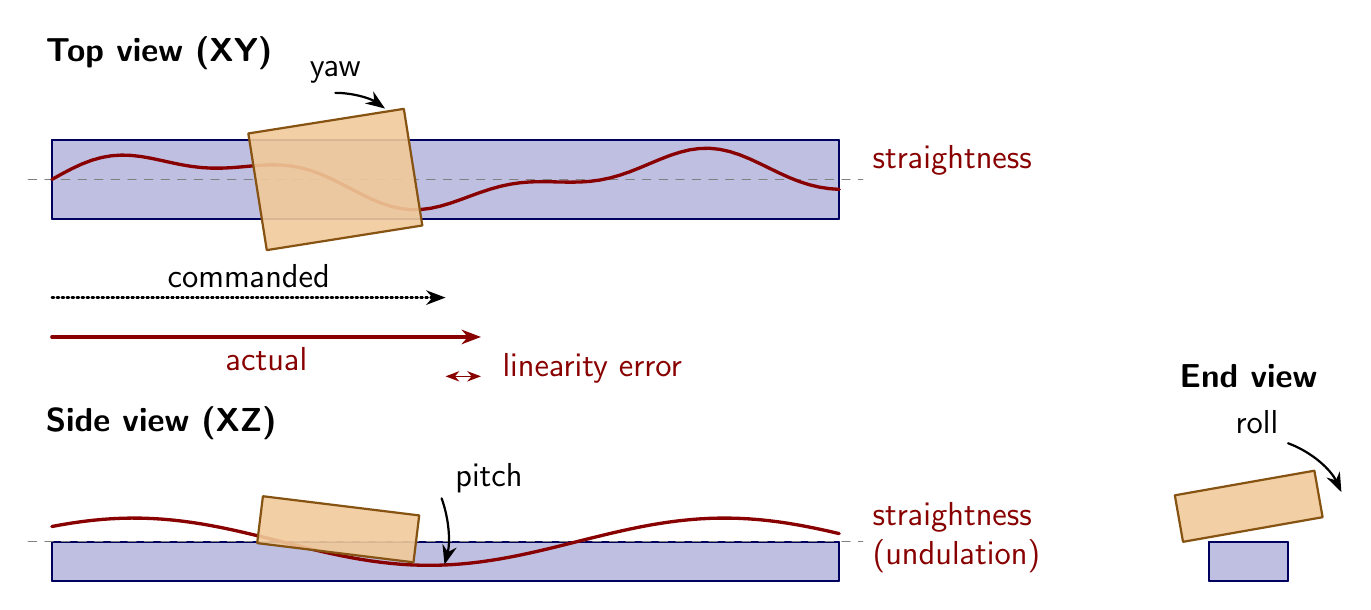
\begin{tikzpicture}[font=\large]
  \tikzset{rail/.style={thick, fill=dmblue!25, draw=dmblue!70!black},
           carr/.style={thick, fill=dmorange!45, draw=dmorange!60!black, fill opacity=0.9},
           err/.style={dmred, very thick}}
  % ---- top view (XY): yaw and straightness in Y
  \begin{scope}
    \node[anchor=west, font=\large\bfseries] at (-0.2,2.1) {Top view (XY)};
    \fill[rail] (0,0) rectangle (10,1); \draw[rail] (0,0) rectangle (10,1);
    \draw[dashed, gray] (-0.3,0.5) -- (10.3,0.5);
    \draw[err, domain=0:10, samples=80] plot (\x, {0.5+0.28*sin(\x*55)+0.12*sin(\x*140)});
    \draw[carr, rotate around={9:(3.6,0.5)}] (2.6,-0.25) rectangle (4.6,1.25);
    \node[dmred, anchor=west] at (10.3,0.75) {straightness};
    \draw[->, thick] (3.6,1.6) arc[start angle=90, end angle=55, radius=1.1];
    \node[above] at (3.6,1.6) {yaw};
  \end{scope}
  % ---- linearity: commanded vs actual displacement
  \begin{scope}[yshift=-1.3cm]
    \draw[->, thick, densely dotted] (0,0.3) -- node[above] {commanded} (5,0.3);
    \draw[->, err] (0,-0.2) -- node[below] {actual} (5.45,-0.2);
    \draw[dim, dmred] (5,-0.7) -- (5.45,-0.7);
    \node[dmred, anchor=west] at (5.6,-0.6) {linearity error};
  \end{scope}
  % ---- side view (XZ): pitch and straightness in Z (undulation)
  \begin{scope}[yshift=-4.6cm]
    \node[anchor=west, font=\large\bfseries] at (-0.2,2.0) {Side view (XZ)};
    \fill[rail] (0,0) rectangle (10,0.5); \draw[rail] (0,0) rectangle (10,0.5);
    \draw[dashed, gray] (-0.3,0.5) -- (10.3,0.5);
    \draw[err, domain=0:10, samples=80] plot (\x, {0.5+0.3*sin(\x*48+40)});
    \draw[carr, rotate around={-7:(3.6,0.36)}] (2.6,0.36) rectangle (4.6,0.96);
    \node[dmred, anchor=west, align=left] at (10.3,0.55) {straightness\\(undulation)};
    \draw[->, thick] (4.95,1.05) arc[start angle=20, end angle=-15, radius=1.4];
    \node[right] at (5.0,1.3) {pitch};
  \end{scope}
  % ---- end view (YZ): roll
  \begin{scope}[shift={(15.2,-4.6)}]
    \node[anchor=west, font=\large\bfseries] at (-1.0,2.6) {End view};
    \fill[rail] (-0.5,0) rectangle (0.5,0.5); \draw[rail] (-0.5,0) rectangle (0.5,0.5);
    \draw[carr, rotate around={10:(0,0.95)}] (-0.9,0.65) rectangle (0.9,1.25);
    \draw[->, thick] (0.5,1.75) arc[start angle=70, end angle=25, radius=1.2];
    \node[above left] at (0.5,1.75) {roll};
  \end{scope}
\end{tikzpicture}
\end{document}
